\documentclass[11pt]{article}

\usepackage[margin=1in]{geometry}
\usepackage{amsmath, amssymb}
\usepackage{graphicx}
\usepackage{booktabs}
\usepackage{caption}
\usepackage{hyperref}
\usepackage{float}

\title{MGT 595: Quantitative Investing \\ Problem Set 1}
\author{Group: Ashley Wen, Emily Wu, Grace Gu}
\date{\today}

\begin{document}
\maketitle

\setcounter{section}{-1}

\section{Dataset Construction}

\subsection{Investment Philosophy}

\textbf{What investment philosophy guided the construction of the universe?}

This portfolio was constructed with a focus on ``Quality Growth.'' Because of
our shared interest in Information Technology and Health Care, we assigned
greater weights to these sectors for their long-term growth potential and
profitability. We also allocated a meaningful share to Energy, where structural
demand and different economic drivers could help balance the growth-oriented
holdings. Meanwhile, the portfolio maintains exposure to all 11 GICS sectors
to reduce concentration risk and avoid relying too heavily on the performance
of only a few industries.

\subsection{Candidate Pool and Screening Method}

\textbf{How were the stocks screened and selected?}

Once the number of stocks required from each sector had been determined, we
formed a candidate pool approximately twice the size of the eventual
allocation. The candidate pools included both large, established companies
and smaller firms with market capitalizations below \$5 billion.

We then compared the candidates using a simplified multifactor framework that
considered profitability, revenue growth, valuation, leverage, price momentum,
and market risk. Because the portfolio follows a ``Quality Growth'' philosophy,
greater emphasis was placed on growth and profitability. Valuation, debt,
\texttt{Beta}, and recent price movements were also considered to keep the
overall risk at a reasonable level.

\subsection{Final Stock Universe}

\textbf{Does the final universe satisfy the assignment requirements?}

The final universe contains exactly 50 U.S.-listed stocks and maintains
exposure across all 11 GICS sectors. It includes five companies with market
capitalizations below \$5 billion: \texttt{OII}, \texttt{ADUS}, \texttt{LNN},
\texttt{PLUS}, and \texttt{PLAB}. Therefore, the universe satisfies both the
sector-diversification and small-cap requirements of the assignment.

After the stocks had been selected, the 50 tickers were alphabetized before
constructing the nested portfolios used in Part 1. The first 5, 10, and 25
stocks were therefore determined by this fixed alphabetical order rather than
by their screening rankings. This makes the comparison across portfolio sizes
more neutral by preventing us from intentionally placing our most preferred
stocks in the smaller portfolios.

\subsection{Data Collection}

\textbf{How were the historical prices obtained?}

Adjusted monthly closing prices for all 50 stocks and the S\&P 500
(\texttt{\^{}GSPC}) were downloaded using \texttt{yfinance} with
\texttt{interval="1mo"} and \texttt{auto\_adjust=True}. The final sample covers
January 2010 through the most recent complete month and contains 200 monthly
return observations.

\subsection{Missing-Data Validation}

\textbf{Were any stocks or months removed because of missing data?}

All 50 stocks had complete monthly coverage over the common sample period.
Therefore, no ticker exceeded the assignment's 5\% missing-data threshold, no
ticker was dropped or replaced, and no month was removed during complete-case
alignment.

\subsection{Extreme-Return Validation}

\textbf{Were potentially unusual monthly returns investigated?}

As part of the data-validation process, monthly returns below $-50\%$ or above
$+200\%$ were flagged for investigation rather than automatically removed.
Three observations met this criterion: \texttt{EXEL} returned approximately
$-63.0\%$ in September 2014, while \texttt{OII} and \texttt{OKE} each declined
by approximately $70\%$ in March 2020.

The latter two observations coincided with the COVID-19 market disruption and
the collapse in oil prices. Because the flagged observations appeared to
represent genuine market movements rather than data errors, they were retained
in the final dataset.

\subsection{Bias Acknowledgement}

\textbf{How should selection and survivorship bias affect the interpretation
of the results?}

Our sample is subject to both selection and survivorship bias. The selection
process intentionally favored companies with stronger current fundamentals,
particularly in Information Technology and Health Care. As a result, the
portfolio's returns, volatility, and covariance structure may not be
representative of the broader U.S. stock market.

In addition, requiring continuous historical data back to January 2010
restricted the sample to companies that are still listed today. Firms that
failed, were delisted, or were acquired before the selection date were excluded
by construction. Therefore, average returns may appear higher and downside risk
may appear lower than they would in a universe that included unsuccessful
firms, although this effect is not guaranteed for every excluded company.

The diversification patterns reported in Part 1 should consequently be
interpreted as evidence for this particular group of selected surviving firms,
rather than as general estimates for all stocks that were investable in January
2010. Alphabetizing the tickers makes the comparison among the nested
portfolios more neutral, but it does not eliminate the selection bias in the
original 50-stock universe.

\subsection{Dataset Summary}

\begin{itemize}
    \item \textbf{Investment philosophy:} Quality Growth
    \item \textbf{Number of stocks:} 50
    \item \textbf{GICS sectors represented:} 11
    \item \textbf{Stocks below \$5 billion:} 5
    \item \textbf{Market benchmark:} S\&P 500 (\texttt{\^{}GSPC})
    \item \textbf{Return frequency:} Monthly
    \item \textbf{Final number of monthly returns:} 200
    \item \textbf{Stocks dropped or replaced:} None
    \item \textbf{Months removed during alignment:} None
    \item \textbf{Extreme observations flagged and retained:} 3
\end{itemize}

% =====================================================================
\section{Part 1: Diversification and Basic Statistics}
% =====================================================================

\subsection{Question 1(a): Diversification and Basic Statistics}

We form equal-weight portfolios using the first 5, 10, 25, and all 50
tickers in fixed alphabetical order. For each portfolio, the sample mean and
sample standard deviation of monthly returns were computed.

\begin{table}[H]
\centering
\caption{Equal-weight portfolio statistics}
\begin{tabular}{cccc}
\toprule
$N$ & Sample Mean & Sample Std.\ Dev. \\
\midrule
5  & 1.6362\% & 4.9518\% \\
10 & 1.6393\% & 4.4471\% \\
25 & 1.5201\% & 4.5803\% \\
50 & 1.5960\% & 4.4970\% \\
\bottomrule
\end{tabular}
\end{table}

\begin{figure}[H]
\centering
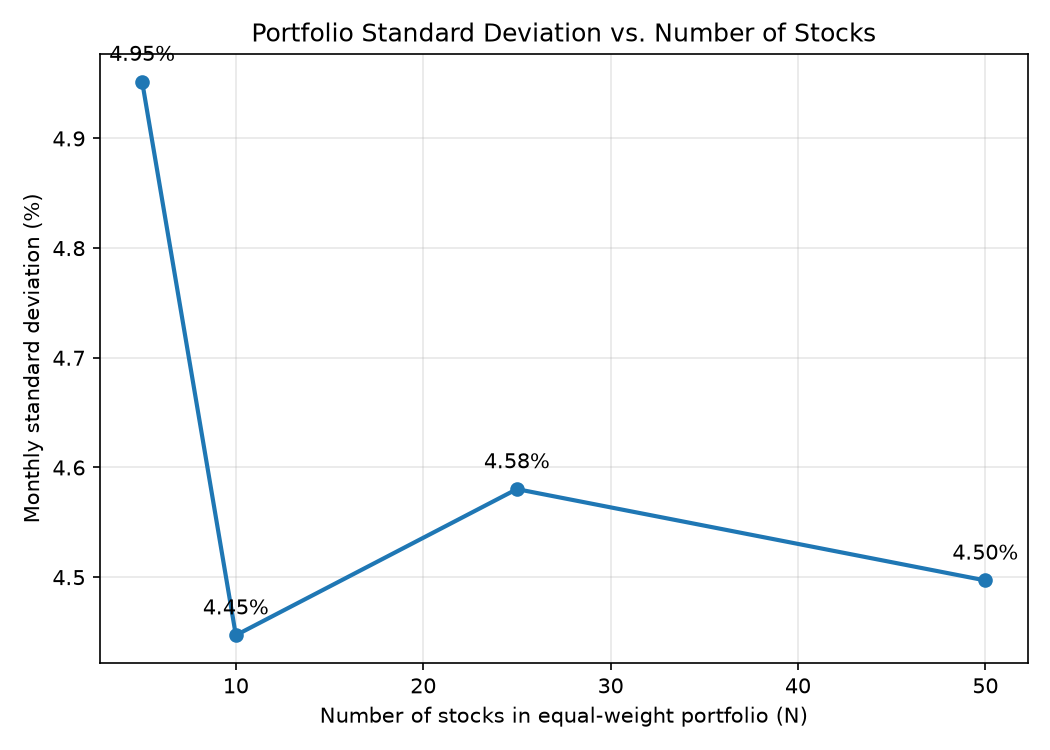
\includegraphics[width=0.75\textwidth]{1a_diversification_curve.png}
\caption{Portfolio standard deviation vs.\ number of stocks ($N$)}
\end{figure}

\paragraph{Discussion.} Although the curve is not perfectly monotonic, it shows an overall downward and flattening pattern. This is broadly consistent with diversification theory: adding stocks generally reduces firm-specific risk, but a realized nested sample does not guarantee that volatility falls with every addition.

Despite the decline, the standard deviation would not reach zero even if the porfolio grows larger. As the portfolio becomes larger, firm-specific risk declines, butcommon covariance and systematic market risk remain and cannot be diversified
away.

\subsection{Question 1(b): Variance Decomposition}

For each equal-weight portfolio, we decomposed total variance into a
contribution from individual stock variances and a contribution from
covariances, using
\[
\mathrm{Var}(r_p) = \frac{1}{N}\,\overline{\mathrm{Var}} +
\frac{N-1}{N}\,\overline{\mathrm{Cov}},
\]
where $\overline{\mathrm{Cov}}$ is backed out algebraically from the
portfolio variance and the average individual variance, without directly
estimating the full pairwise covariance matrix.

\begin{table}[H]
\centering
\caption{Variance decomposition by portfolio size}
\begin{tabular}{ccccccc}
\toprule
$N$ & Avg.\ Var. & Avg.\ Cov. & Port.\ Var. & Var.\ Contrib. & Cov.\ Contrib. & \% from Var. \\
\midrule
5  & 0.007284 & 0.001244 & 0.002452 & 0.001457 & 0.000995 & 59.41\% \\
10 & 0.006481 & 0.001477 & 0.001978 & 0.000648 & 0.001330 & 32.77\% \\
25 & 0.007113 & 0.001889 & 0.002098 & 0.000285 & 0.001813 & 13.56\% \\
50 & 0.007485 & 0.001911 & 0.002022 & 0.000150 & 0.001873 & 7.40\% \\
\bottomrule
\end{tabular}
\end{table}

\begin{figure}[H]
\centering
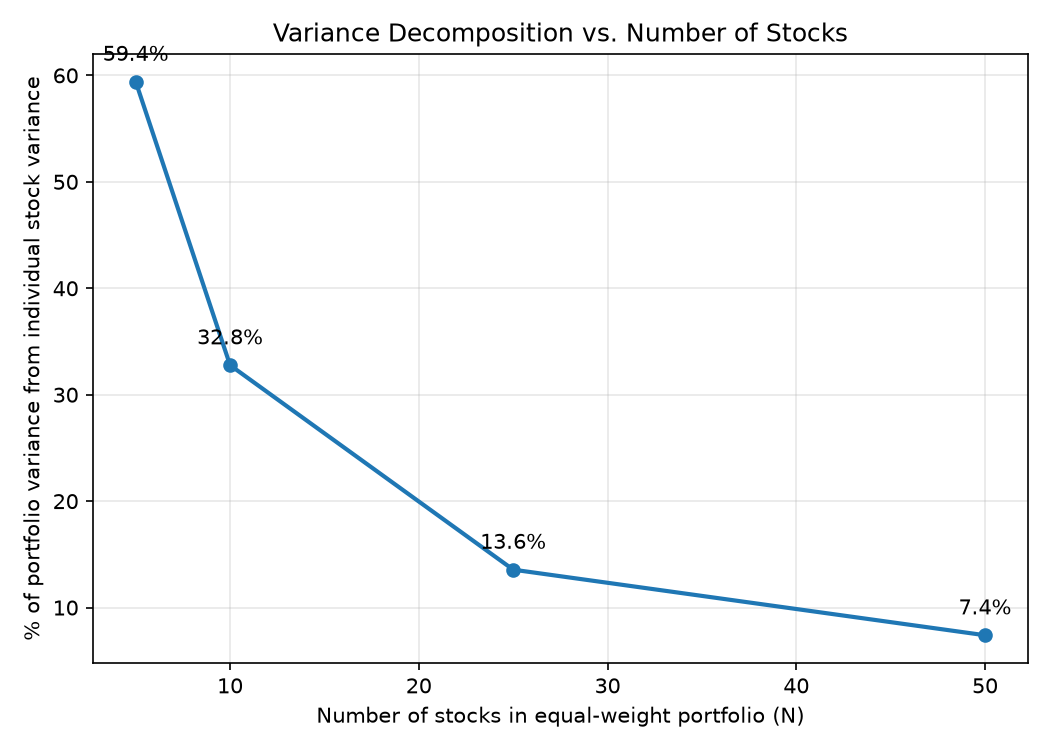
\includegraphics[width=0.75\textwidth]{1b_variance_decomposition.png}
\caption{Percentage of portfolio variance from individual stock variance vs.\ $N$}
\end{figure}

\paragraph{Discussion.} Compared with Question 1(a), this curve shows a much
smoother decline. As the number of stocks increases, the percentage of
portfolio variance attributable to individual stock variances decreases,
making the covariance contribution increasingly important.

This is consistent with diversification theory. Because the
individual-variance component is divided by $N^2$, it is gradually diluted as
the portfolio grows and may approach zero. However, total portfolio variance
does not approach zero because covariance persists as stocks remain exposed to
shared market and economic conditions.

\subsection{Question 1(c): Value-Weighted vs.\ Equal-Weighted Variance}

A value-weighted portfolio would likely have lower variance if larger-cap stocks are less volatile and not highly correlated with each other. Variance could be higher if the portfolio becomes concentrated in a few large firms that are more volatile or move closely together. In Part (b), most of our 50-stock portfolio variance came from covariance rather than individual stock variances. This suggests that changing from equal weighting to value weighting would mainly affect variance through changes in the covariance structure and concentration of the portfolio.

\subsection{Question 1(d): Hypothesis Testing on Portfolio Mean Returns}

We test the null hypothesis for each equal-weighted portfolio. Since the population variance is unknown and estimated using the sample standard deviation, the test statistic follows a Student's $t$-distribution with $T-1 = 199$ degrees of freedom.

\begin{table}[H]
\centering
\caption{$t$-statistics for portfolio mean returns}
\begin{tabular}{lrrrl}
\toprule
Portfolio & Mean Monthly Return & $t$-statistic & $p$-value & Conclusion \\
\midrule
5 stocks  & 0.016362 & 4.673 & $<0.0001$ & Reject $H_0$ \\
10 stocks & 0.016393 & 5.213 & $<0.0001$ & Reject $H_0$ \\
25 stocks & 0.015201 & 4.693 & $<0.0001$ & Reject $H_0$ \\
50 stocks & 0.015960 & 5.019 & $<0.0001$ & Reject $H_0$ \\
\bottomrule
\end{tabular}
\end{table}

At the 5\% significance level, we reject the null hypothesis for all four portfolios. The results provide strong evidence that the mean monthly return of each portfolio is statistically different from zero. All four estimated mean returns are positive.

\subsection{Question 1(e): Jarque--Bera Normality Test}

We use the Jarque--Bera test to test the null hypothesis that returns are normally distributed.

\begin{table}[H]
\centering
\caption{Jarque--Bera test results}
\begin{tabular}{lrrrrl}
\toprule
Series & Skewness & Excess Kurtosis & JB Statistic & $p$-value & Conclusion \\
\midrule
AAPL & $-0.0299$ & $-0.3549$ & 1.0796 & 0.5829 & Fail to reject normality \\
50-stock portfolio & $-0.2128$ & 0.7776 & 6.5479 & 0.0379 & Reject normality \\
S\&P 500 & $-0.3351$ & 0.6041 & 6.7856 & 0.0336 & Reject normality \\
\bottomrule
\end{tabular}
\end{table}

At the 5\% significance level, we fail to reject normality for AAPL, but reject normality for both the 50-stock portfolio and the S\&P 500. AAPL is nearly symmetric and has slightly negative excess kurtosis, while the portfolio and the market both have negative skewness and positive excess kurtosis, indicating heavier tails.

\paragraph{AI Integration.} The LLM explained that positive excess kurtosis indicates fatter tails than a normal distribution, meaning extreme returns occur more frequently than a Gaussian model predicts. It also noted that normal-parametric VaR may therefore underestimate tail risk.

The LLM's interpretation of excess kurtosis is reasonable. Both the 50-stock portfolio and the S\&P 500 have positive excess kurtosis and reject normality, suggesting that a Gaussian VaR model may understate the probability of extreme losses.

However, our results do not show that diversification necessarily makes returns more normal. AAPL fails to reject normality, while both the diversified portfolio and the S\&P 500 reject it. Although the central limit theorem suggests that diversification can make idiosyncratic components more normally distributed, common market shocks and correlated movements can prevent the portfolio from becoming fully normal.

\subsection{Question 1(f): Market Regressions for Ten Stocks}

We regress the monthly returns of ten stocks on the monthly return of the S\&P 500.

\begin{table}[H]
\centering
\caption{OLS regressions of individual stock returns on the S\&P 500}
\begin{tabular}{lrrrrr}
\toprule
Stock & Alpha & Alpha SE & Beta & Beta SE & $R^2$ \\
\midrule
AAPL  & 0.0112 & 0.0044 & 1.1056 & 0.1042 & 0.3624 \\
ABT   & 0.0029 & 0.0036 & 0.7135 & 0.0835 & 0.2695 \\
ADBE  & 0.0009 & 0.0049 & 1.2124 & 0.1156 & 0.3571 \\
ADUS  & 0.0154 & 0.0091 & 0.4807 & 0.2143 & 0.0248 \\
AMGN  & 0.0070 & 0.0044 & 0.6282 & 0.1038 & 0.1561 \\
AMZN  & 0.0089 & 0.0051 & 1.2505 & 0.1202 & 0.3534 \\
CAT   & 0.0049 & 0.0050 & 1.3828 & 0.1182 & 0.4088 \\
CMCSA & $-0.0001$ & 0.0040 & 0.9638 & 0.0928 & 0.3528 \\
COST  & 0.0094 & 0.0033 & 0.7156 & 0.0775 & 0.3011 \\
CSCO  & 0.0012 & 0.0042 & 1.0854 & 0.0990 & 0.3777 \\
\bottomrule
\end{tabular}
\end{table}

\paragraph{Interpretation.} A beta above 1 means that the stock tends to move more than the market. For example, CAT has the highest beta at 1.3828, indicating relatively high sensitivity to market movements. In contrast, stocks such as ADUS, AMGN, ABT, and COST have betas below 1 and therefore tend to respond less strongly to market movements.

Alpha represents the average return not explained by exposure to the S\&P 500. A positive alpha indicates a positive average return beyond that predicted by the market regression, while a negative alpha indicates the opposite. Most stocks in our sample have positive estimated alphas, while CMCSA's alpha is approximately zero.

$R^2$ measures how much of a stock's return variation is explained by movements in the S\&P 500. CAT has the highest $R^2$ at 0.4088, meaning about 41\% of its monthly return variation is explained by the market. ADUS has a very low $R^2$ of 0.0248, suggesting that its returns are driven mainly by firm-specific or other factors rather than broad market movements.

% =====================================================================
\section{Part 2: Rolling Estimates}
% =====================================================================

We choose NVIDIA (\texttt{NVDA}) as our stock of interest for the rolling-window analyses below.

\subsection{Question 2(a): Expanding vs.\ Rolling Volatility}

For NVDA and the S\&P 500, we calculate monthly return volatility using an expanding window and a 12-month rolling window.

\begin{table}[H]
\centering
\caption{Final expanding and 12-month rolling volatility estimates}
\begin{tabular}{lcc}
\toprule
Series & Expanding Volatility & 12-Month Rolling Volatility \\
\midrule
NVDA     & 0.1278 & 0.0785 \\
S\&P 500 & 0.0415 & 0.0383 \\
\bottomrule
\end{tabular}
\end{table}

\begin{figure}[H]
\centering
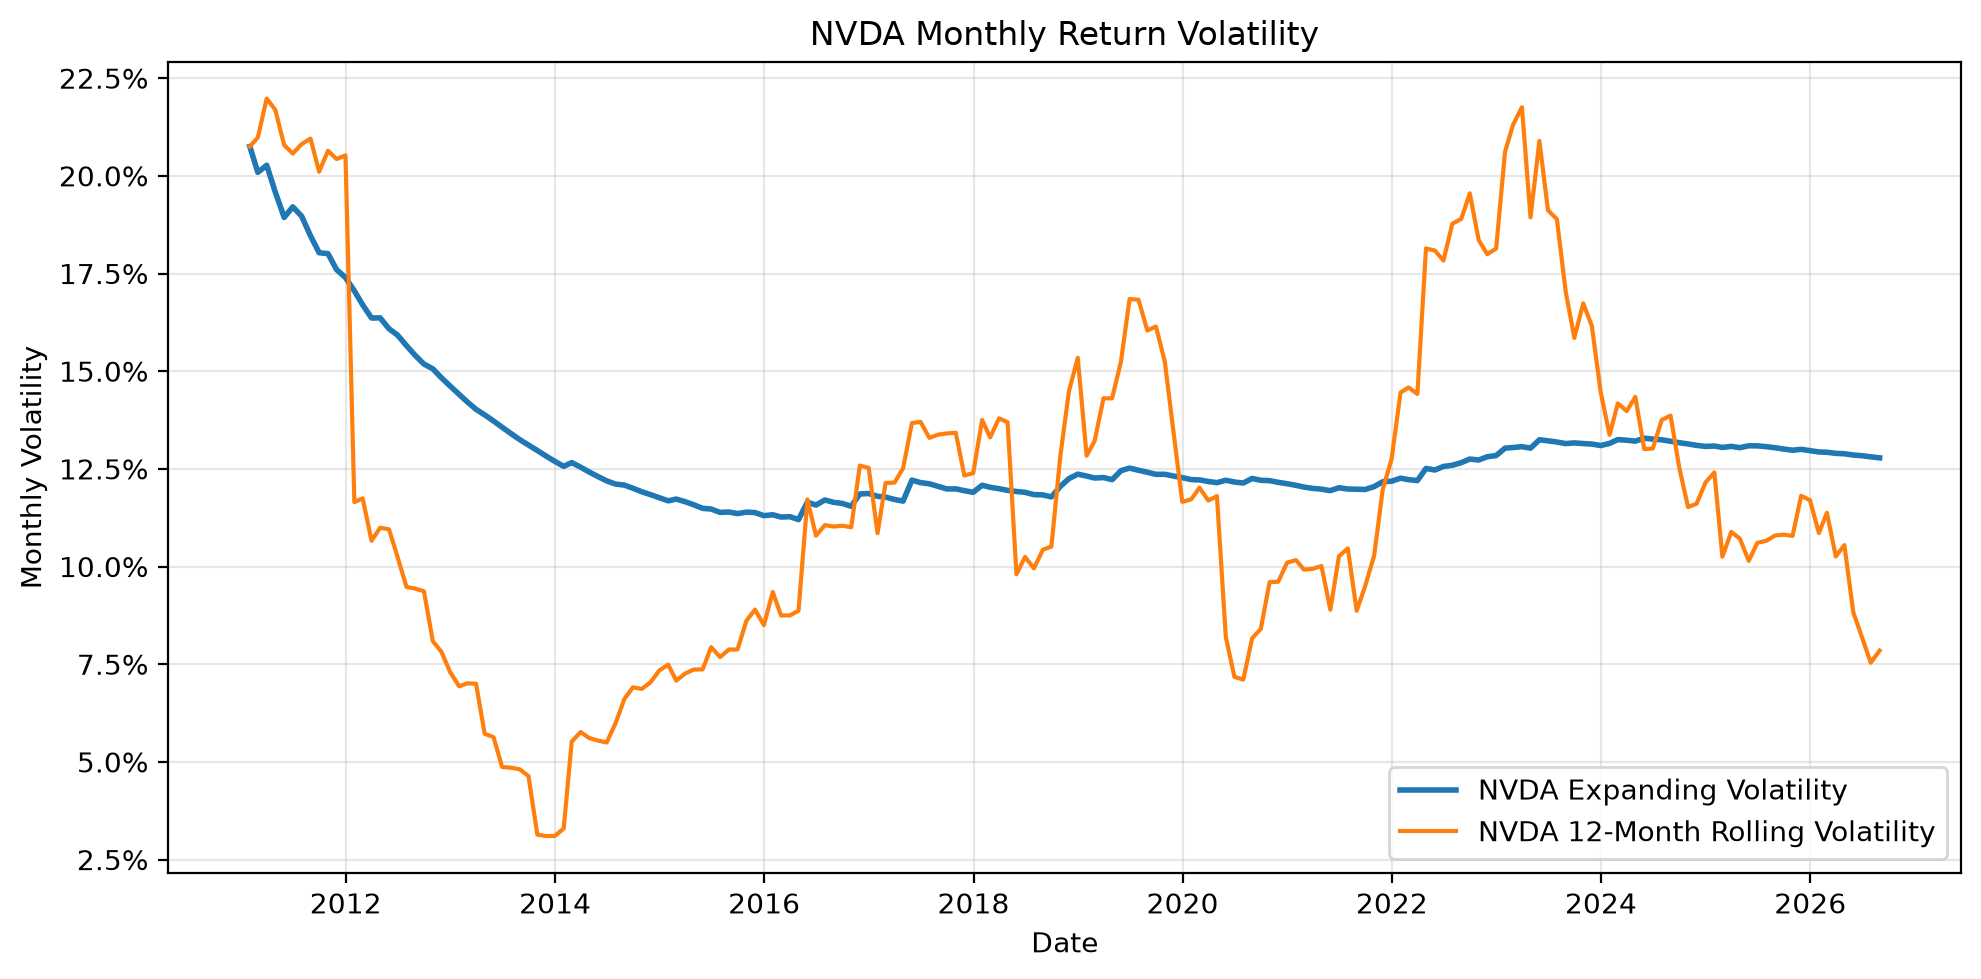
\includegraphics[width=0.75\textwidth]{Part2/2a_nvda_volatility.png}
\caption{Expanding and 12-month rolling monthly volatility for NVDA.}
\end{figure}

\begin{figure}[H]
\centering
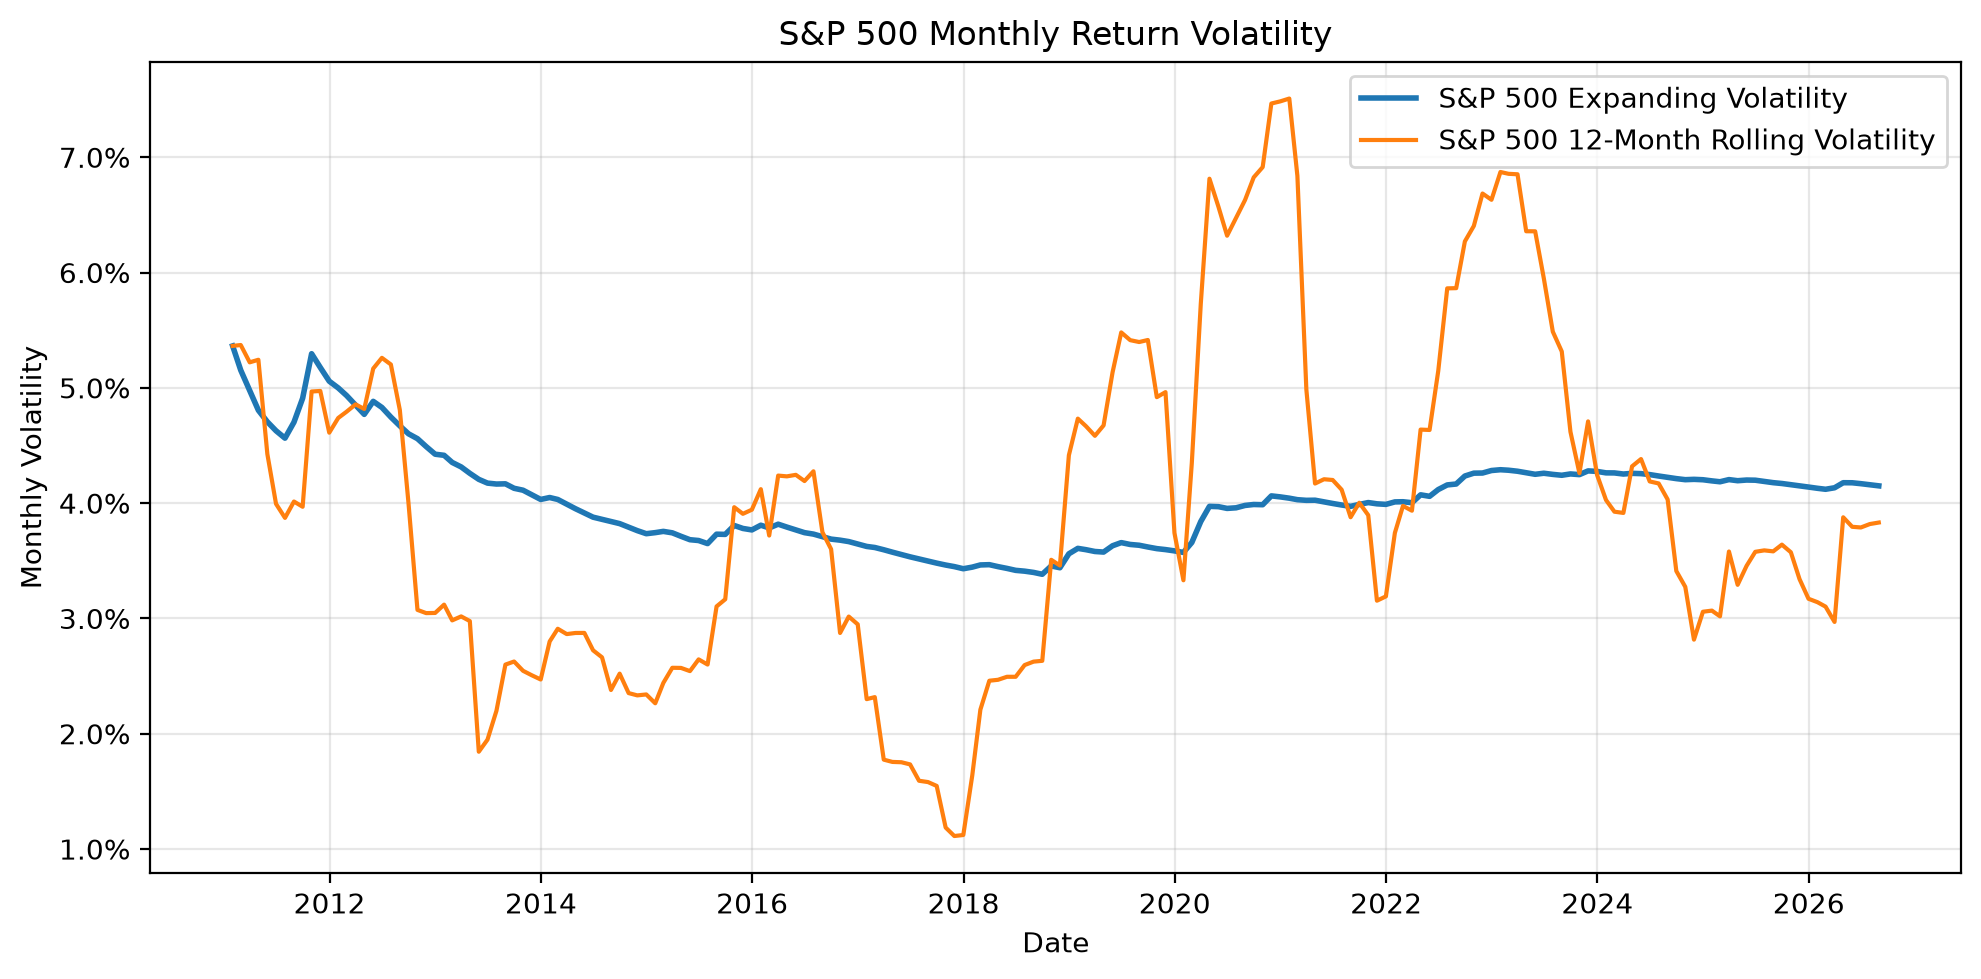
\includegraphics[width=0.75\textwidth]{Part2/2a_sp500_volatility.png}
\caption{Expanding and 12-month rolling monthly volatility for the S\&P 500.}
\end{figure}

\paragraph{Interpretation.} For NVDA and the S\&P 500 Index, the 12-month rolling volatility estimates fluctuate much more widely than the expanding-window estimates. NVDA's rolling volatility changes particularly strongly over the sample, while its expanding-window volatility gradually stabilizes as more observations are incorporated. The S\&P 500 shows the same general pattern, although its volatility is lower than NVDA's.

There are two reasons why the rolling estimates fluctuate more. First, each rolling estimate uses only 12 monthly observations, making it more susceptible to sampling error and individual extreme returns. Second, the rolling window continuously adds the most recent observation and removes the oldest observation, so it reacts rapidly to changes in the recent volatility environment. In contrast, the expanding estimate uses all available observations up to each date, so the influence of any single observation declines as the sample becomes larger.

\subsection{Question 2(b): Expanding vs.\ Rolling Beta}

We estimate NVDA's OLS beta relative to the S\&P 500 using both an expanding window and a 12-month rolling window. The chart also reports 95\% confidence intervals for each beta estimate.

\begin{table}[H]
\centering
\caption{Full-sample beta and extremes of the 12-month rolling beta}
\begin{tabular}{lll}
\toprule
Measure & Estimate & Date / Interval \\
\midrule
Full-sample beta     & 1.7144  & 95\% CI: [1.3549, 2.0739] \\
Minimum rolling beta & $-2.0985$ & 2017-11-30 \\
Maximum rolling beta & 3.1190  & 2026-02-28 \\
\bottomrule
\end{tabular}
\end{table}

\begin{figure}[H]
\centering
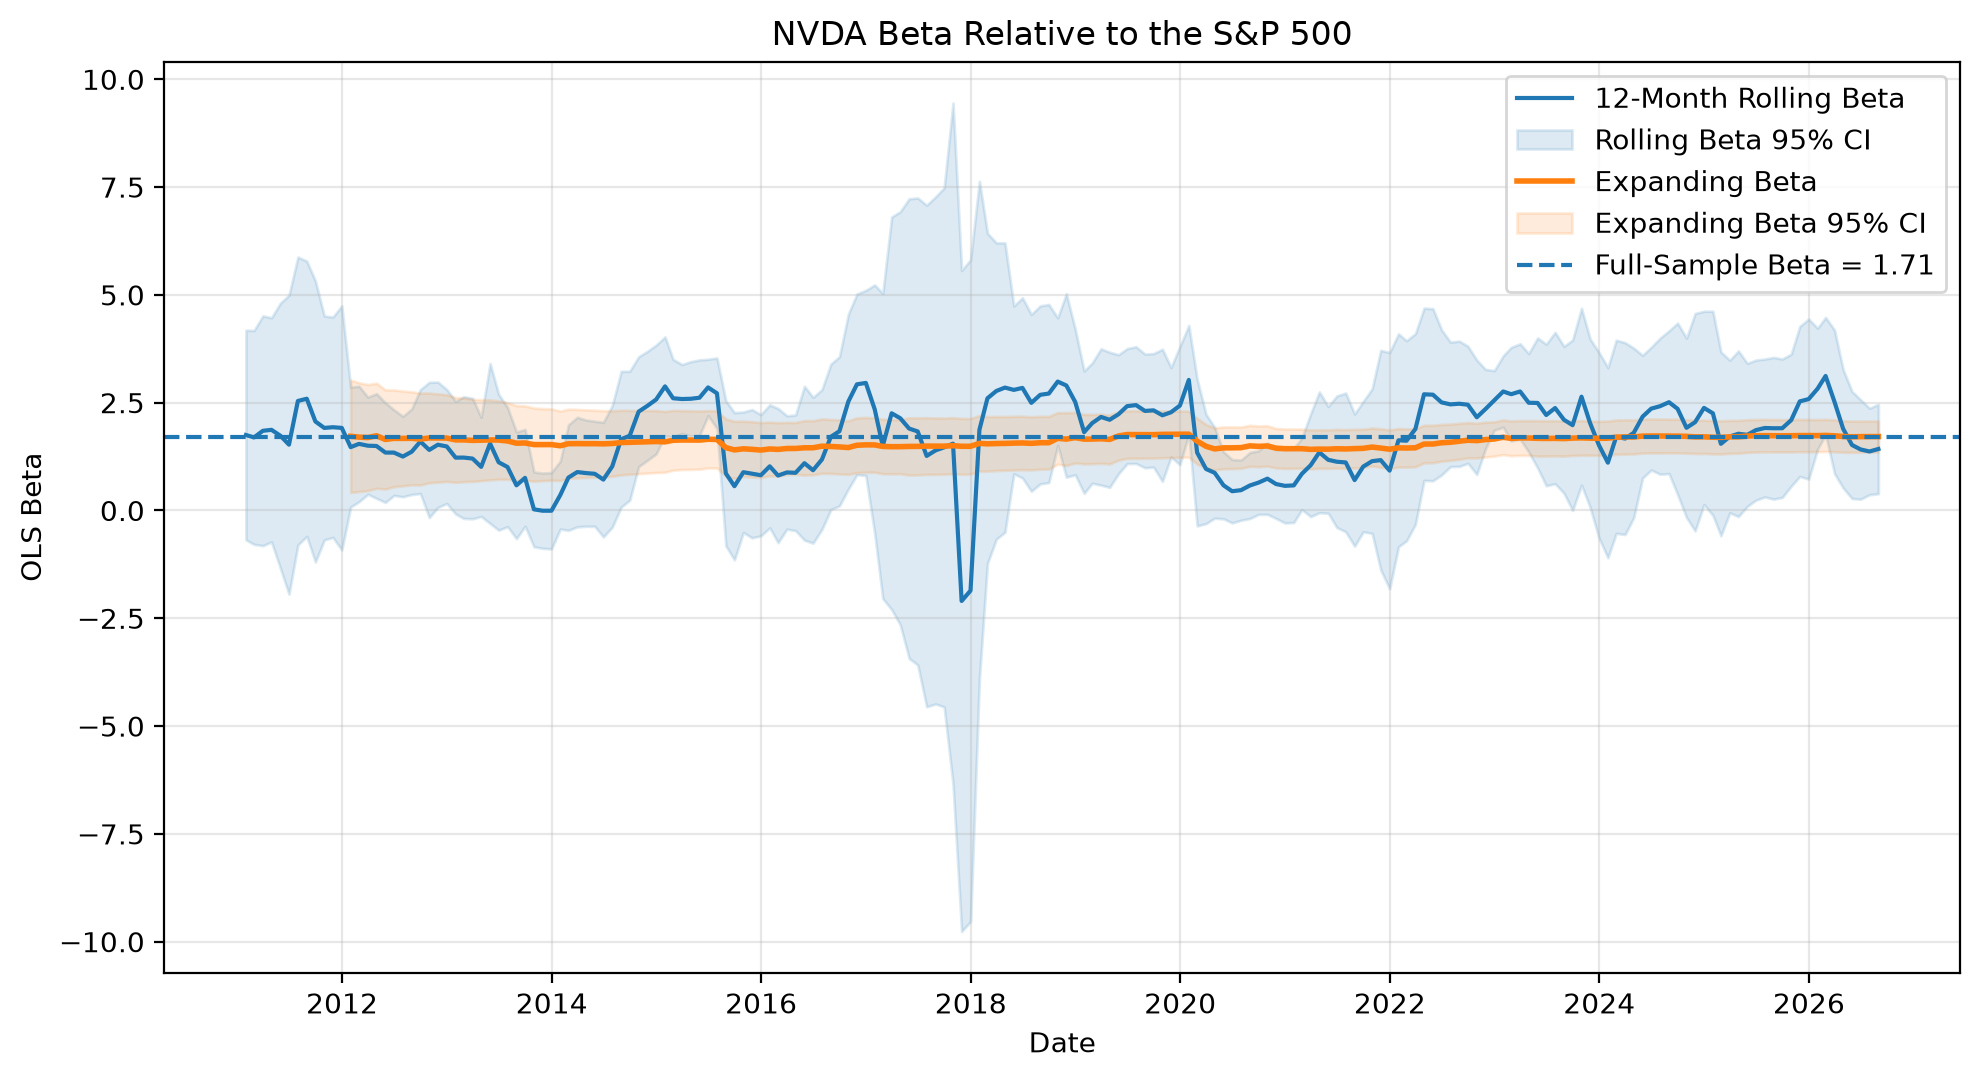
\includegraphics[width=0.75\textwidth]{Part2/2b_rolling_beta.png}
\caption{NVDA expanding and 12-month rolling beta relative to the S\&P 500, with 95\% confidence intervals.}
\end{figure}

\paragraph{Interpretation.} NVDA's 12-month rolling beta varies substantially over time, ranging from approximately $-2.10$ to $3.12$, compared with a full-sample beta of 1.71 and a 95\% confidence interval of $[1.35, 2.07]$. However, this does not necessarily mean that NVDA's true beta varies dramatically over time. Each rolling regression uses only 12 monthly observations and therefore has only 10 residual degrees of freedom, making the estimates noisy and producing wide confidence intervals. The chart may therefore reflect both genuine changes in market-risk exposure and substantial short-window estimation error.

\paragraph{AI Integration --- Rolling Beta.}
\textit{Prompt:} My one-year rolling OLS beta for NVDA fluctuates between $-2.0985$ and $3.1190$ over the sample, while the full-sample estimate is $1.7144$ with a 95\% confidence interval of $[1.3549, 2.0739]$. Does this imply that true beta is time-varying, or is sampling error a more plausible explanation?

\textit{Answer from LLM:} The wide range of one-year rolling beta estimates does not by itself imply that NVIDIA's true beta is time-varying. Because each rolling regression uses only 12 observations and estimates both an intercept and slope, it has only 10 residual degrees of freedom, so sampling uncertainty can be substantial. Wide confidence intervals around many of the rolling estimates would indicate that these estimates are imprecise and that large apparent changes may arise even if the underlying beta were relatively stable. Genuine time variation is still possible, particularly if NVIDIA's business exposure or sensitivity to market-wide shocks changed, but stronger evidence than the movement of the point estimates alone would be needed to distinguish structural change from estimation noise.

\textit{Evaluation:} The LLM's answer is mostly correct. It correctly distinguishes possible genuine time variation in beta from estimation uncertainty caused by the short 12-month window. It also correctly explains that wide confidence intervals indicate that the beta estimates are imprecise; they do not by themselves prove that the true beta changed. However, the response is somewhat general because it does not discuss NVDA's actual behavior during an identifiable episode such as the 2020 COVID crash.

\paragraph{COVID-19 Episode.} During 2020, NVDA's 12-month rolling beta fell substantially. The minimum rolling beta during the March--December 2020 period was 0.45 on 2020-06-30, compared with NVDA's full-sample beta of 1.71. This indicates that NVDA's returns during that particular 12-month window exhibited less estimated sensitivity to contemporaneous S\&P 500 returns than its long-run beta would suggest. One possible economic explanation is that NVDA's business exposure during the COVID shock differed from that of many firms in the broader market.

At the same time, the 95\% confidence interval around the 2020-06-30 rolling-beta estimate is approximately $[-0.29, 1.18]$. Because this interval is wide, the decline should not be treated as conclusive evidence of a structural change in NVDA's true beta. Substantial sampling uncertainty remains because the regression contains only 12 monthly observations.

% =====================================================================
\section*{Exhibit: Final Ticker List and Sector Assignments}
% =====================================================================

\begin{table}[H]
\centering
\caption{Final 50-stock universe by ticker, sector, and company name}
\small
\begin{tabular}{lll}
\toprule
Ticker & GICS Sector & Company Name \\
\midrule
AAPL  & Information Technology  & Apple Inc. \\
ABT   & Health Care             & Abbott Laboratories \\
ADBE  & Information Technology  & Adobe Inc \\
ADUS  & Health Care             & Addus HomeCare Corp \\
AMGN  & Health Care             & AMGEN Inc \\
AMZN  & Consumer Discretionary  & Amazon.com, Inc. \\
CAT   & Industrials             & Caterpillar Inc. \\
CMCSA & Communication Services  & Comcast Corp \\
COST  & Consumer Staples        & Costco Wholesale \\
CSCO  & Information Technology  & Cisco Systems \\
CVX   & Energy                  & Chevron Corp \\
DIS   & Communication Services  & Walt Disney Co. \\
ECL   & Materials               & Ecolab Inc. \\
EMR   & Industrials             & Emerson Electric \\
EOG   & Energy                  & EOG Resources Inc \\
EXEL  & Health Care             & Exelixis Inc \\
FFIV  & Information Technology  & F5 Inc \\
GD    & Industrials             & General Dynamics Corp \\
GE    & Industrials             & GE Aerospace (General Electric) \\
GOOGL & Communication Services  & Alphabet Inc. \\
GS    & Financials              & Goldman Sachs Group Inc. \\
HD    & Consumer Discretionary  & Home Depot Inc \\
INCY  & Health Care             & Incyte Corp \\
JNJ   & Health Care             & Johnson \& Johnson \\
JPM   & Financials              & JPMorgan Chase \& Co \\
KO    & Consumer Staples        & Coca-Cola Co. \\
LNN   & Industrials             & Lindsay Corp. \\
MCD   & Consumer Discretionary  & McDonald's Corp. \\
MDT   & Health Care             & Medtronic Plc \\
MS    & Financials              & Morgan Stanley \\
MSFT  & Information Technology  & Microsoft Corp. \\
MU    & Information Technology  & Micron Technology Inc \\
NEE   & Utilities               & NextEra Energy Inc. \\
NTAP  & Information Technology  & Netapp Inc \\
NVDA  & Information Technology  & NVIDIA Corp \\
OII   & Energy                  & Oceaneering International Inc \\
OKE   & Energy                  & Oneok Inc \\
PG    & Consumer Staples        & Procter \& Gamble Co \\
PH    & Industrials             & Parker-Hannifin Corp \\
PLAB  & Information Technology  & Photronics Inc. \\
PLD   & Real Estate             & Prologis Inc. \\
PLUS  & Information Technology  & ePlus Inc \\
QCOM  & Information Technology  & Qualcomm Inc \\
REGN  & Health Care             & Regeneron Pharmaceuticals Inc \\
SHW   & Materials               & Sherwin-Williams Co \\
TJX   & Consumer Discretionary  & TJX Companies Inc \\
TXN   & Information Technology  & Texas Instruments \\
UNH   & Health Care             & Unitedhealth Group Inc \\
UNP   & Industrials             & Union Pacific Corp \\
WMT   & Consumer Staples        & Walmart Inc. \\
\bottomrule
\end{tabular}
\end{table}

\end{document}
